\section{Specific Requirements}\label{sec requirements}

\subsection{External Interface Requirements}

\subsubsection{User interfaces}

The user interfaces must satisfy the following UI constraints:
\begin{itemize}
	\item Web application
	\begin{enumerate}
		\item The web pages must adhere to the W3C standards. In particular, the software shall conform to the HTML~5~\cite{w3c-html5}, CSS~\cite{w3c-css} standards.
	\end{enumerate}
	\item Mobile application
	\begin{enumerate}
		\item The iOS version must adhere to the iOS Human Interface Guidelines~\cite{apple-ios-hig}.
		\item The Android version must follow Android design guidelines~\cite{google-android-hig}.
	\end{enumerate}
		\item Common to web and mobile applications:
		\begin{enumerate}
			\item The client applications must have an UI that is accessible to disabled people.
			\item The interface must offer the possibility to choose the language used at all times.
			\item The first screen must ask the user to login in order to begin operations.
			\item UI controls and views must be suitable for the input interface and the screen size.
		\end{enumerate}
	\item Car application
	\begin{enumerate}
		\item Radio and navigation applications must be implemented.
		\item A Label on the screen will always notify the driver about the current cost of the ride.
	\end{enumerate}
	\item Server back-end
	\begin{enumerate}
		\item The server back-end must be configurable by means of a configuration text file.
	\end{enumerate}
	
\subsubsection{Hardware interfaces}
The embedded system of any vehicles must be provided of	
\begin{itemize}
	\item a 7" touchscreen display
	\item a GPS device
	\item sensors that check if all the parts of the car are working correctly
	\item sensors that check how many passengers are on the car
	\item a 4G router for a stable Internet connection
	\item a secondary battery used only if the main battery is discharged. The vehicle can't use this battery
\end{itemize}

\subsubsection{Software interfaces}
The required software products used by the back-end are:
\begin{itemize}
	\item MySQL 5.7\footnote{\url{http://dev.mysql.com}}
	\item Java SE 8\footnote{\url{http://www.oracle.com/technetwork/java/javase/overview/index.html}}
\end{itemize}
The required software product used by the car application is:
\begin{itemize}
	\item Java Embedded\footnote{\url{http://www.oracle.com/technetwork/java/embedded/overview/index.html}}
\end{itemize}
The required operating systems for the mobile application atr:
\begin{itemize}
	\item iOS 8 or more recent
	\item Android 6.0 or more recent
\end{itemize}

For a detailed specification of the programmatic interfaces, see \autoref{sec:api}.
	
\subsubsection{Communications interfaces}
The clients communicate with the server via HTTPS requests (port 443).

\end{itemize}

\subsection{System Features}

\subsubsection{Driver registration}

\paragraph{Purpose}
Any guest can subscribe through web or mobile applications.

In both cases the guest has to fill a registration form and must agree to the personal data policy according to his/her country privacy laws, otherwise the registration request shall be aborted.

As soon as the guest has submitted all the data, the system verifies the consistency of the information and a confirmation mail with a password is sent to the email address indicated in the registration form. The guest 
must confirm his/her email address for end the registration.

Once registered a guest can be recognized as a driver through the login phase.

\paragraph{Scenario 1}
Bob, a normal citizen without a car, has just discovered the existence of the PowerEnJoy Service and he wants to use it.

He opens the homepage of PowerEnJoy website and procedes to the registration clicking on the button "sign up".

He gives all the information required and authorises the personal data treatment. 

The system verifies all the informations that bob submitted to the form and sends a confirmation mail to him.

Bob checks his mailbox, opens the mail and clicks on "Confirm email". He is also notified about his current password.

The system informs Bob that he is successfully registered.

\begin{figure}[H]
	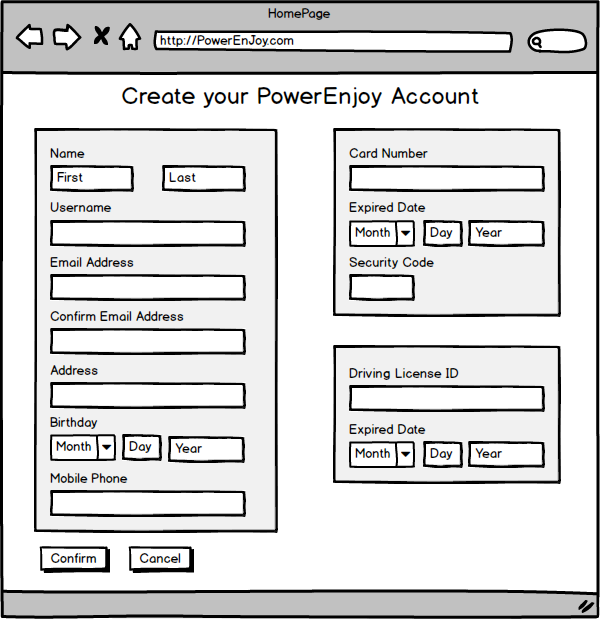
\includegraphics[width=\textwidth]{mockup/WebRegistration.png}
	\caption{Concept of the registration webpage.}
\end{figure}

\begin{figure}[H]
	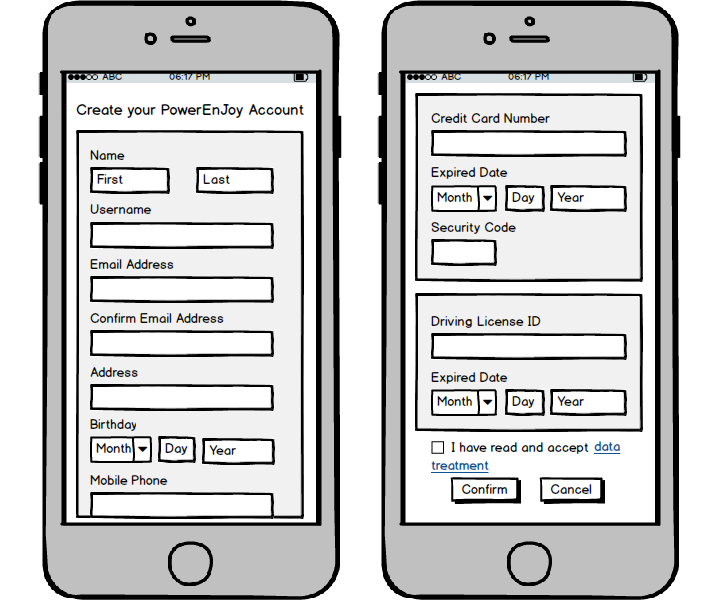
\includegraphics[width=\textwidth]{mockup/MobileRegistration.png}
	\caption{Concept of the mobile registration.}
\end{figure}

\paragraph{Use case description}

\paragraph{Associated functional requirements}

\subsection{Performance Requirements}

\subsection{Software System Attributes}

\subsection{Alloy}